\chapter{Opis interfejsu systemu}
\section{Moduł silnika i symulatora gry}
\subsection{Główne okno aplikacji}
\begin{par}
Podstawowym oknem aplikacji widocznym tuż po uruchomieniu jest główne okno symulatora gry. 
Domyślnym trybem jest tryb poruszania się po mapie przez użytkownika. 
Sterowanie postacią przez klawiaturę zrealizowanie jest za pomocą strzałek kierunkowych, oraz klawiszy $a,s,d,f$ jako akcji specjalnych.
Reakcja środowiska na poszczególne klawisze zależy od logiki gry, domyślnie jest to logika reprezentowana przez klasę LogicMario (strzałki kierunkowe odpowiadają za ruch postaci, natomiast klawisz f za skok).
Poniżej przedstawiony został opis poszczególnych elementów menu.
\begin{figure}[!h]
		\centering
		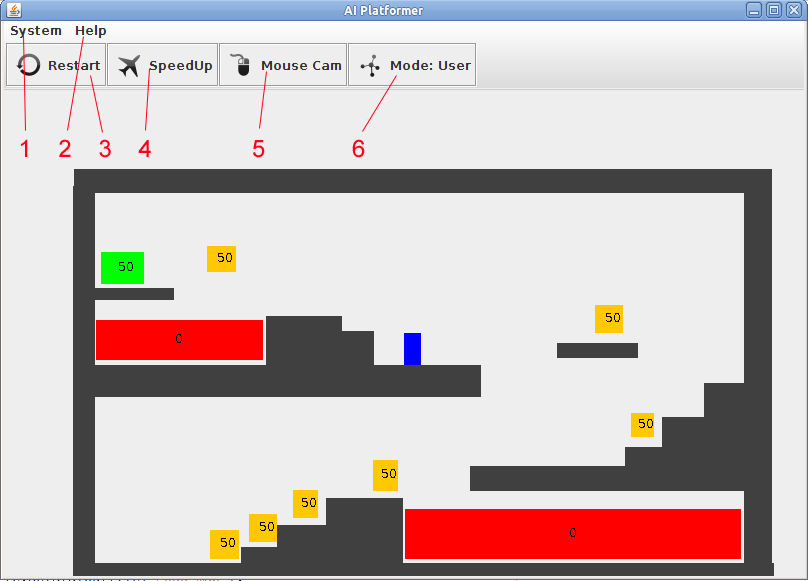
\includegraphics[width=4in]{obrazki/main_window.png}
		\caption{Główne okno aplikacji.}
		\label{fig:main_window}
	\end{figure}
W oknie aplikacji widoczne jest menu oraz pasek narzędzi zawierający podstawowe przyciski sterujące systemem:
	\begin{enumerate}
	\item Z menu ``System'' użytkownik ma możliwość otwarcia dodatkowych okien aplikacji takich jak edytor map, panel ustawień, podgląd populacji oraz menu dialogowe dotyczące wczytania nowej mapy z pliku do środowiska gry.
	\item Menu ``Help'' zawiera informacje dotyczące programu oraz krótki opis skrótów klawiszowych.
	\item Przycisk ``Restart'' pozwala na ponowne uruchomienie algorytmu, czyli wygenerowanie losowej populacji.
	\item Przycisk ``SpeedUp'' odpowiada za przejście systemu w tryb treningu przyspieszonego, jeśli populacja aktualnie znajduje się w trybie treningu. Przestaje wówczas być aktualizowana grafika, a system w tle symuluje kolejne populacje osobników w środowisku gry.
	\item Domyślnym trybem kamery jest śledzenie obiektu aktora. Przycisk ``Mouse Cam'' pozwala na przejście w tryb swobodnej kamery - prawy przycisk myszy służy do ``przesuwania'' ekranu.
	\item Przycisk ``Mode: User''(``Mode: Genetic'') służy do zmiany trybu działania systemu. Domyślnie pierwszym trybem jest tryb poruszania się po mapie przez użytkownika. Po wciśnięciu przycisku system przechodzi do trybu treningu populacji. Kolejne wciśnięcie przycisku przywraca poprzedni tryb swobodnego poruszania się.
	\end{enumerate}
	\FloatBarrier
\end{par}
\begin{par}
	Środowisko gry znajduje się w centralnej części okna gry.
	Wszystkie elementy gry z punktu widzenia kolizji są prostokątnymi obszarami, różniącymi się reakcją na kolizję z obiektem gracza. W podstawowym silniku renderującym zostały one wyróżnione kolorem.
	
	\definecolor{orange}{rgb}{1,0.5,0}
	\definecolor{gray}{rgb}{0.5,0.5,0.5}
	Na Rys. \ref{fig:objects} widać obiekty świata gry: 
	\textcolor{blue}{\textit{Actor}}, 
	\textcolor{orange}{\textit{BonusCoin}},
	\textcolor{red}{\textit{BonusLose}},
	\textcolor{green}{\textit{BonusWin}},
	\textcolor{black}{\textit{Terrain}}.

	\begin{figure}[!h]
		\centering
		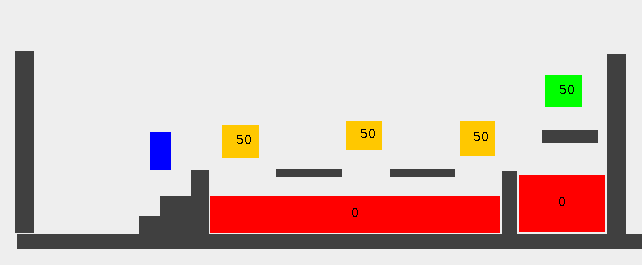
\includegraphics[width=4in]{obrazki/objects.png}
		\caption{Poszczególne obiekty świata gry.}
		\label{fig:objects}
	\end{figure}
\end{par}
\subsection{Panel konfiguracyjny}
\begin{par}
	Jak już zostało wspomniane, podstawą dobrego systemu, szczególnie do zastosowań badawczych jest łatwo dostępna konfiguracja. 
	W pracy rolę tę pełni pośrednio klasa \textit{GeneticsConfig} która zawiera wszystkie najważniejsze parametry dotyczące algorytmu. Są przechowywane jako wartości tablicy asocjacyjnej (klasa \textit{HashMap}). 
	Oprócz tego sama tablica została opakowana w taki sposób iż rejestracja nowej wartości do tablicy wiąże się z automatycznym wygenerowaniem odpowiedniego pola w panelu konfiguracyjnym - dzięki temu dodanie kolejnych parametrów genetycznych przy przyszłym rozbudowywaniu aplikacji automatycznie aktualizuje panel konfiguracyjny.
\end{par}
\begin{par}
	Każda z akcji, zarówno ruchu jak i tablica akcji specjalnych posiada pewne prawdopodobieństwo wystąpienia.
	Zostały one podzielone na dwie grupy: \textit{Movement key probabilities} oraz \textit{Special key probabilities}
	Wartości te możliwe są do zmiany w panelu konfiguracyjnym, przy czym są one normalizowane do sumy wszystkich wartości z danej kategorii.
	Przykładowo dla wartości podanych na rys \ref{fig:config1}. Wartość ruchu w prawo (grupa ``Movement key probabilities'') wynosi $\frac{2.5}{2.5+0.5+0.2}=0.78125$.
	Aby nie brać pod uwagę akcji które i tak nie będą interpretowane przez logikę, najlepiej jest ustawić prawdopodobieństwo wylosowania ruchów nieaktywnych na wartość $0$. 
	Mapa gry może być ukierunkowana bądź nie, wówczas ustawienie odpowiedniego stosunku akcji ruchu może znacznie przyspieszyć znalezienie wyniku. Przykładowo: Jeśli problemem jest znalezienie rozwiązania na szerokiej mapie, której cel znajduje się w jej prawym krańcu, dobrą strategią będzie ustawienie ruchu w prawo na wysoką wartość np. $0.95$ a ruchu w lewo na wartość $0.05$.
	\begin{figure}[!h]
		\centering
		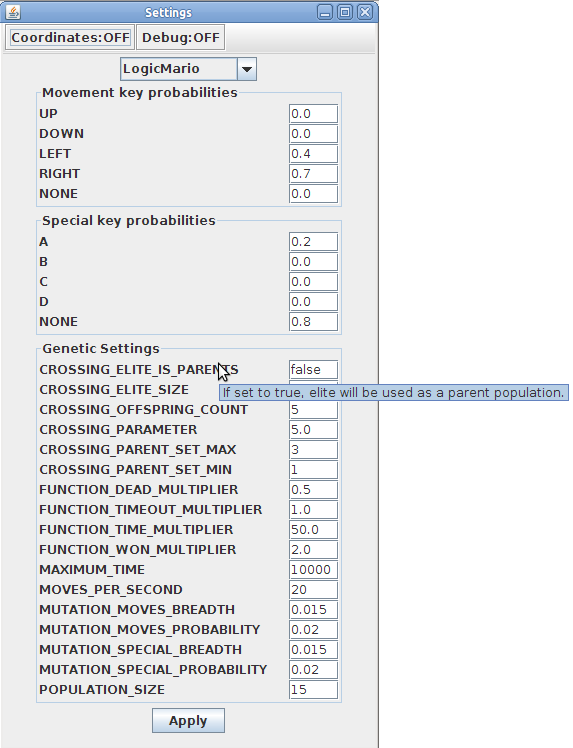
\includegraphics[width=4in]{obrazki/config1.png}
		\caption{Panel Konfiguracyjny.}
		\label{fig:config1}
	\end{figure}
	Trzecia grupa parametrów są to parametry algorytmu genetycznego (grupa \textit{Genetic Settings}). Po umieszczeniu kursora myszy nad nazwą parametru wyświetlany jest jego opis słowny. Uzytkownik może zmienić poszczególne parametry. W wypadku zmiany parametrów wymagających ponownego uruchomienia aplikacji, wyświetlone zostaje okno pytające o potwierdzenie operacji.
	\newline
	Ponieważ algorytm genetyczny jest niezależny od stosowanej logiki gry, możliwe jest rozbudowywanie aplikacji o dodawanie własnych klas dziedziczących po klasie Logic. Użytkownik ma możliwość zmiany logiki w panelu ustawień, za pomocą listy na górze okna ustawień.
	Dwa dodatkowe przyciski w panelu konfiguracyjnym (``Coordinates'' oraz ``Debug'') służą do włączenia wyświetlania informacji o obiektach takich jak ich położenie w przestrzeni, lub informacji o stanie gry. Mogą one okazać się przydatne przy tworzeniu własnych map, bądź pisaniu własnej logiki gry.
\end{par}
\subsection{Widok Populacji i Chromosomu}
\begin{par}
	Podczas działania algorytmu genetycznego nawet w trybie przyspieszonym, użytkownik może śledzić postępy w oknie ``Population'' dostępnym z menu (Rys. \ref{fig:populacja}).
	Zawiera ono listę aktualnie dostępnych osobników w populacji i wyświetla krótkie podsumowanie dotyczące przebiegu danego osobnika w symulacji gry. Kolejno \textit{Result} oznacza wynik końcowy po zakończeniu przebiegu, \textit{Score} dotyczy sumy wszystkich zebranych punktów na mapie. Wartość \textit{Time} oznacza czas przebiegu danego chromosomu w milisekundach.
	Ostatecznie \textit{Final Score} jest wartością funkcji przystosowania przeliczoną przez algorytm. Jeśli dany osobnik jeszcze nie wziął udziału w przebiegu gry, wyświetlany jest komunikat ``State not Set''. Po zaznaczeniu dowolnego osobnika użytkownik ma możliwość tymczasowego uruchomienia przejścia za pomocą przycisku ``Run selected gene''. Po zaznaczeniu osobnika i wciśnięciu przycisku ``Show details'' wyświetlane zostaje okno podglądu chromosomu - Rys. \ref{fig:chromosom}.

	\begin{figure}[!h]
		\centering
		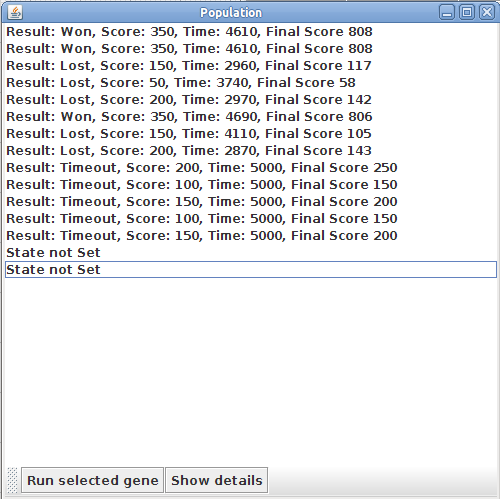
\includegraphics[width=4in]{obrazki/populacja.png}
		\caption{Okno populacji.}
		\label{fig:populacja}
	\end{figure}


	\begin{figure}[!h]
		\centering
		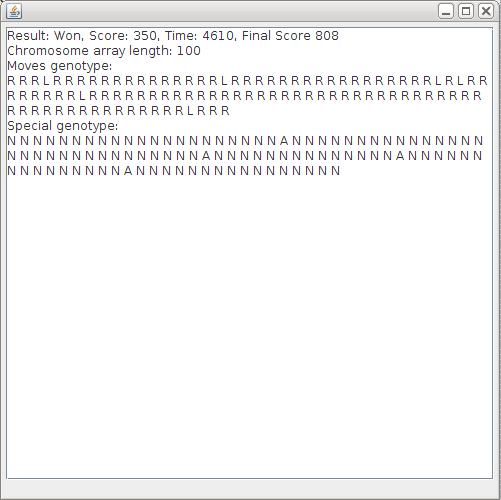
\includegraphics[width=4in]{obrazki/chromosom.png}
		\caption{Okno szczegółów chromosomu.}
		\label{fig:chromosom}
	\end{figure}
	\FloatBarrier
\end{par}
\begin{par}
	Podstawową logiką gry i detekcją kolizji pomiędzy obiektami zarządza obiekt klasy \textit{Logic}. Użytym w pracy schematem logiki jest schemat gry ``Super Mario Brothers''. Wobec czego domyślną logiką gry przy uruchomieniu programu jest instancja klasy \textit{LogicMario}.
	Zakłada ona ruch w 2 kierunkach, skok oraz działanie grawitacji na obiekt aktora.
	Ponieważ klasa \textit{LogicMario} dziedziczy po klasie \textit{Logic} możliwe jest napisanie własnej logiki i podmiana tej obowiązującej w systemie.
	Inną logiką gry dostępną w systemie jest klasa LogicLabirynth: zakłada ona ruch postaci w 4 kierunkach, akcje specjalne nie są używane.
	Ponieważ działanie algorytmu nie jest związane z fizyką ani zasadami obowiązującymi w grze, system może działać dla wielu różnych typów gier platformowych i zręcznościowych.
	Jedynym wymogiem jest to iż muszą one dać się opisać za pomocą wyżej zdefiniowanych klas i cech:
	\begin{enumerate}
		\item
			Obiekty świata muszą należeć do którejś z klas dziedziczących po klasie \textit{WorldObject}.
		\item 
			Możliwe rezultaty zakończenia algorytmu muszą być wśród zbioru rezultatów: \{Koniec Czasu, Wygrana, Przegrana\}, 
		\item
			Rodzaje możliwych akcji do wykonania w grze muszą być przypisane do 4 akcji ruchu kierunkowego oraz 4 akcji specjalnych.
	\end{enumerate}

	Jedyną pracą jaką należy wykonać przy implementacji własnego środowiska gry jest uzupełnienie własnej klasy dziedziczącej po klasie \textit{Logic}.
	Wówczas przy poprawnej implementacji logiki gry system automatycznie symuluje zbiory chromosomów w środowisku gry.
\end{par}

\subsection{Edytor Map}
\begin{par}
Przy testowaniu różnych ustawień algorytmu genetycznego przydatnym narzędziem może okazać się edytor map. 
Ustawienia algorytmu, szczególnie dotyczące prawdopodobieństwa wylosowania akcji w dużej mierze zależą od typu mapy. 
\begin{par}
	Użytkownik może otworzyć okno edytora map wybierają opcję ``Map Editor'' z menu głównego okna aplikacji.
	Po otworzeniu edytora map domyślnie wczytywana jest bieżąca mapa z symulatora gry, dzięki czemu można dokonać szybkich edycji jeśli koniecznie jest sprawdzenie działania algorytmu z pewnym wariantem, lub dodatkowym obiektem na mapie.
	Oprócz tego wszystkie mapy zapisywane są w prostym formacie tekstowym, dzięki czemu możliwe jest generowanie map przy pomocy programów trzecich, lub skryptów - zostawia to furtkę dla bardziej zaawansowanych użytkowników na generowanie dużych poziomów, lub wykorzystanie algorytmów tworzących losowe tereny.
	Przykładowy plik z mapą może wyglądać następująco:
	\begin{lstlisting}
		Terrain 122 361 239 27
		Terrain 110 211 25 151
		Terrain 355 201 28 165
		Actor 140 295 20 32
		BonusCoin 202 328 18 30 25
		BonusCoin 248 330 16 27 25
		BonusWin 327 236 18 36 25
		BonusLose 313 311 33 40 0
	\end{lstlisting}

	Pierwszym elementem każdego wiersza jest nazwa klasy.
	Kolejne wartości to punkt oznaczający położenie lewego górnego rogu obiektu, oraz jego szerokość i wysokość.
	W wypadku obiektów klasy \textit{Bonus} ostatnia liczba oznacza wartość punktową. 
	Ponieważ nie było powodu aby przechowywać mapy jako dane binarne - samo wczytywanie mapy nie spowalnia aplikacji oraz nie jest wykonywane często - otwarty format pozostał jako obowiązujący w systemie.
\end{par}
\begin{par}
	\begin{figure}[!h]
	\centering
	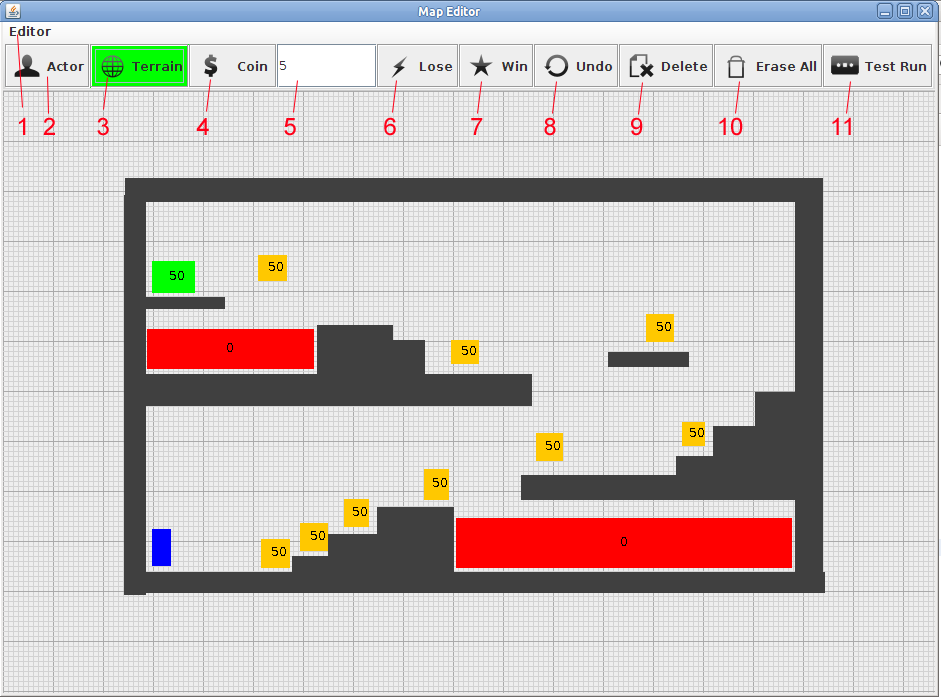
\includegraphics[width=5.5in]{obrazki/map_editor.png}
	\caption{Okno edytora map.}
	\label{fig:map_editor}
	\end{figure}
	Samo okno edytora map składa się z menu oraz paska narzędzi. Posługiwanie się większością narzędzi jest podobne:
	\begin{itemize}
	\item Użytkownik aby narysować obszar wybiera odpowiedni typ obiektu z paska narzędzi, a następnie trzymając lewy przycisk myszy, wyznacza prostokątny obszar.
	\item Po kliknięciu na dowolny obiekt lewym przyciskiem myszy, zostaje on zaznaczony, dzięki czemu użytkownik może łatwo usuwać z mapy niepotrzebne obiekty.
	\item Prawy przycisk myszy służy do przesuwania mapy - analogicznie do trybu ``MouseCam'' w module symulacyjnym.
	\end{itemize}
	Poniżej zostaną opisane poszczególne elementy edytora.
	\begin{enumerate}
		\item Menu edytora pozwalające użytkownikowi na wczytanie mapy z pliku, bądź zapis bieżącej mapy do pliku na dysku. W obu przypadkach wyświetlane jest okno dialogowe potwierdzające operację.
		\item Przycisk uaktywniający obiekt aktora. Po wybraniu przycisku obiekty tworzone przez użytkownika będą obiektami aktora. Na mapie jednocześnie może być utworzonych wiele obiektów aktora. Ponieważ w założeniach nie jest powiedziane iż gra może zawierać tylko jeden obiekt sterowany przez użytkownika istnieje możliwość dodania na mapie wielu aktorów - możliwe jest napisanie logiki wykorzystującej więcej niż jeden obiekt aktora.
		\item Obiekt Terrain odpowiada za statyczny teren gry. O ile interpretacja kolizji aktora z obiektem tego typu jest pozostawiona do interpretacji dla twórcy logiki, to głównym założeniem obiektu Terrain miało być ograniczanie ruchu postaci po mapie.
		\item Przycisk Coin odpowiada za umieszczanie obiekty BonusCoin dających punkty.
		\item Wartość w polu tekstowym pozwala na ustalenie wartości jaką ma mieć następny stworzony przez użytkownika obiekt BonusCoin.
		\item Przycisk Lose odpowiada za umieszczanie na mapie obiektów typu BonusLose.
		\item Przycisk Win odpowiada za umieszczanie na mapie obiektów typu BonusWin.
		\item Przycisk Undo usuwa ostatnio stworzony obiekt z mapy.
		\item Przycisk Delete usuwa aktualnie zaznaczony na mapie obiekt.
		\item Jeśli użytkownik chce usunąć wszystkie elementy z mapy i rozpocząć tworzenie mapy od początku, może użyć do tego przycisku Erase All który usuwa wszystkie obiekty z edytora map. Przed wykonaniem akcji użytkownik zatwierdza akcję w oknie dialogowym.
		\item Przycisk Test Run służy do załadowania bieżącej mapy z edytora do środowiska gry. Jeśli aktualnie system pracuje w trybie treningu populacji, konieczne jest rozpoczęcie algorytmu od początku. Mapa zostaje zapisana na dysk jako plik tymczasowy. Przed wykonaniem akcji użytkownik zatwierdza akcję w oknie dialogowym.
		
	\end{enumerate}
\end{par}
	
\end{par}

